\documentclass[tikz,border=2pt]{standalone}
\usepackage{tikz}
\usepackage{pgfplots}
\usetikzlibrary{intersections}
\usetikzlibrary{positioning}
\usetikzlibrary{graphs}

\begin{document}
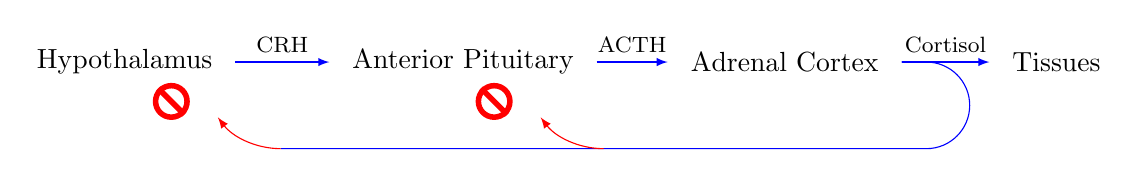
\begin{tikzpicture}
\node[anchor=west,outer sep=5pt](T1)at(-6.6,0){Hypothalamus};
\draw[-latex,blue,](T1)--node[black,above,font=\footnotesize]{CRH}++(2.6,0)
coordinate(PT2);
\node[anchor=west,outer sep=5pt](T2)at(PT2){Anterior Pituitary};
\draw[-latex,blue](T2)--node[black,above,font=\footnotesize]{ACTH}++(2.6,0)
coordinate(PT3);
\node[anchor=west,outer sep=5pt](T3)at(PT3){Adrenal Cortex};
\draw[-latex,blue](T3)--node[black,above,font=\footnotesize]{Cortisol}++(2.6,0)
coordinate(PT4);
\node[anchor=west,outer sep=5pt](T4)at(PT4){Tissues};

\coordinate(W1)at(-4.6,-0.5);
\coordinate(W2)at(-0.5,-0.5);

\node[draw=red,shape=circle,line width=2pt,
minimum height=4mm,inner sep=1pt] (C1)at(W1){};
\draw[red,line width=2pt](C1.315)--(C1.135);

\node[draw=red,shape=circle,line width=2pt,
minimum height=4mm,inner sep=1pt] (C2)at(W2){};
\draw[red,line width=2pt](C2.315)--(C2.135);

\draw[blue](T3)--++(1.8,0)
arc(90:-90:0.55)--++(-8.2,0)coordinate(KST);

\coordinate(S2)at([xshift=41mm]KST);
\draw[red,-latex](KST)arc(270:217:1);
\draw[red,-latex](S2)arc(270:217:1);
\end{tikzpicture}
\end{document}